\documentclass[../main.tex]{subfiles}

\subsection{Feladat}

Készítsünk programot, amellyel az utazó kereskedők problémáját mutatjuk be.
Ebben néhány kereskedő éjszaka ér egy mély szakadék felett átívelő rozoga hídhoz.
Ezen a hídon a sötétben csak lámpával lehet biztonságosan átkelni, de az utazóknak
sajnos mindössze egyetlen lámpájuk van, továbbá egyszerre legfeljebb hárman
juthatnak át, és valakinek vissza kell menni a lámpával a többiekért. A kereskedők
különböző korúak (fiatal, középkorú, idős), ezért eltérő idő kell nekik a hídon való
átkeléshez. Természetesen, amikor többen mennek át egyszerre, akkor a lassúbbhoz
kell igazítani a lépést. Jelenítsük meg a szakadék két partján lévő kereskedőket,
biztosítsuk azt, hogy mindig felváltva tudjunk egyik vagy másik partról 1-3 személyt
kiválasztani, amely átkerül majd a másik oldalra. A program folyamatosan számolja az
átkelés idejét (természetesen nem valós időben, hanem az előre megadott átkelési
idők segítségével).
A program biztosítson lehetőséget új játék kezdésére a fiatal, középkorú és idős
kereskedők számának megadásával (0-tól 5-ig, minimum 3 különböző összeállításból
választva), és ismerje fel, ha vége a játéknak. Ekkor jelenítse meg, milyen idővel
győzött a játékos, majd kezdjen automatikusan új játékot.

\subsection{Elemzés}

A játékot egy játékos játssza, aki kezeli mind a táblán szereplő játékosokat (kereskedők),
mind a játék menetét. A játékos megállíthatja, folytathatja, újrakezdheti a játékot.
A felhasználói esetek közül az új játék kezdése és a beállítások módosítása valójában ugyanaz
a tevékenység, hiszen a kereskedők számának megváltoztatásával változik a játék nehézsége.
Emiatt, ha a felhasználó beállításokat módosít, muszáj neki új játékot kezdenie.

\begin{center}
    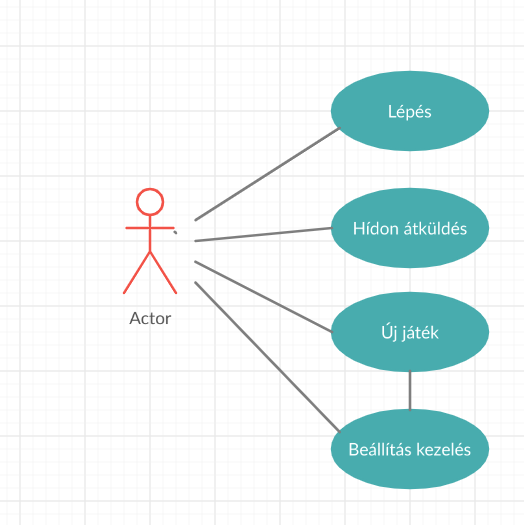
\includegraphics[width= 0.35\textwidth ]{use_cases.png}
\end{center}
    